\chapter{Bayes Theorem for Distributions}
\section{Introduction}
Suppose we have data $\underline{x}$ which we model using the probability
(density) function $f(\underline{x}|\theta)$, which depends on a single
parameter~$\theta$. Once we have observed the data, $f(\underline{x}|\theta)$
is the \textit{likelihood function} for $\theta$ and is a function
of~$\theta$ (for fixed $\underline{x}$) rather than of~$\underline{x}$ (for fixed
$\theta$).

Also, suppose we have prior beliefs about likely values of $\theta$
expressed by a probability (density) function $\pi(\theta)$. We can
combine both pieces of information using the following version of
Bayes Theorem. The resulting distribution for $\theta$ is called the
posterior distribution for~$\theta$ as it expresses our beliefs about
$\theta$ {\it after} seeing the data. It summarises all our current
knowledge about the parameter $\theta$.

\subsection*{Bayes Theorem}
The posterior probability (density) function for $\theta$ is
$$\pi(\theta|\underline{x})=\frac{\pi(\theta)\,f(\underline{x}|\theta)}{f(\underline{x})} 
$$
where
$$
f(\underline{x})=
\begin{cases}
\int_\Theta\pi(\theta)\,f(\underline{x}|\theta)\,d\theta & \text{if
$\theta$ is continuous}, \\ \\
\sum_\Theta\pi(\theta)\,f(\underline{x}|\theta) & \text{if $\theta$ is discrete}.
\end{cases} 
$$
Notice that, as $f(\underline{x})$ is not a function of
$\theta$, Bayes Theorem can be rewritten as
\begin{align*}
\pi(\theta|\underline{x})&\propto \pi(\theta)\times f(\underline{x}|\theta) \\
i.e. \, \text{posterior}&\propto\text{prior}\times\text{likelihood}.
\end{align*}

\newpage

\noindent Thus, to obtain the posterior distribution, we need:
\begin{itemize}
\item [(1)] data, from which we can form the \emph{likelihood} $f(\underline{x}|\theta)$, and 
\item [(2)] a suitable distribution, $\pi(\theta)$, that represents our \emph{prior beliefs} about $\theta$.  
\end{itemize}
You should now be comfortable with how to obtain the likelihood. But how do we specify a prior (point 2)? In Chapter 3 we will consider different approaches to specifying prior distributions.

For now, we will assume someone else has done this for us; the main aim of this chapter is simply to operate Bayes Theorem for distributions to obtain the posterior distribution for $\theta$.  

Before we do this, it will be worth re--familiarising ourselves with some continuous probability distributions you have met before, and which we will use extensively in this course: the uniform, beta and gamma distributions (indeed, I will assume that you are more than familiar with some other `standard' distributions we will use -- e.g. the exponential, Normal, Poisson, and binomial, and so will \textit{not} review these here).  

\paragraph{Definition 2.1: Continuous Uniform distribution}{~\\
The random variable $Y$ follows a Uniform distribution, denoted $U(a,b)$, if it has probability density function
$$
f(y|a,b) = \frac{1}{b-a}, \quad \quad a\leq y \leq b.
$$
This form of probability density function ensures that all values in the range $[a,b]$ are \textit{equally likely}, hence the name ``uniform''.  This distribution is sometimes called the \textit{rectangular distribution} because of its shape.  

You should remember from MAS1608 that 
$$
\text{E}[Y] = \frac{a+b}{2} \quad \text{and} \quad \text{Var}[Y] = \frac{(b-a)^{2}}{12}.
$$}
In the space below, sketch the probability density functions for $U(0,1)$ and $U(10,50)$. 

\paragraph{Plot of Uniform pdfs}{
    
}

\paragraph{Definition 2.2: Beta distribution}{~\\
The random variable $Y$ follows a beta $\textnormal{\text{Beta}}(a,b)$ distribution ($a>0$,
\label{def:beta}
$b>0$) if it has probability density function
\begin{equation}
f(y|a,b)=\frac{y^{a-1}(1-y)^{b-1}}{\mathrm{B}(a,b)},\quad\quad 0<y<1.
\label{eq:betapdf}
\end{equation}
The constant term $\mathrm{B}(a,b)$, also known as the {\it beta function},
ensures that the density integrates to one. Therefore
\begin{equation}
\mathrm{B}(a,b)=\int_0^1
y^{a-1}(1-y)^{b-1}\,dy.
\label{eq:betafn}
\end{equation}
It can be shown that the beta function can be expressed in terms of another function, called the {\it gamma function} $\Gamma(\cdot)$, as
$$
\mathrm{B}(a,b) =\frac{\Gamma(a)\Gamma(b)}{\Gamma(a+b)},
$$
where
\begin{equation}
\label{eq:gammafn}
\Gamma(a)=\int_0^\infty x^{a-1}e^{-x}\,dx.
\end{equation}
Tables are available for both $\mathrm{B}(a,b)$ and $\Gamma(a)$. However, these functions are very simple to evaluate when $a$ and $b$ are integers since the gamma function is a generalisation of the factorial function. In particular, when $a$ and $b$ are integers, we have
$$
\Gamma(a)=(a-1)!\quad\text{and}\quad 
\mathrm{B}(a,b)=\frac{(a-1)!(b-1)!}{(a+b-1)!}.
$$
For example,
\begin{equation*}
\mathrm{B}(2,3)=\frac{1!\times2!}{4!}=\frac{1}{12}.
\end{equation*}
It can be shown, using the identity $\Gamma(a)=(a-1)\Gamma(a-1)$, that
\begin{align*}
\text{E}[Y]&=\frac{a}{a+b},\quad\quad\text{and}\quad\quad 
\text{Var}[Y]=\frac{ab}{(a+b)^2(a+b+1)}. 
\end{align*}
Also,
$$\textnormal{Mode}(Y)=\frac{a-1}{a+b-2}, \quad\text{if $a>1$ and $b>1$}.$$}
\clearpage
\paragraph{Definition 2.3: Gamma distribution}{~\\
  The random variable $Y$ follows a Gamma $\text{Gamma}(a,b)$ distribution
  ($a>0$, $b>0$) if it has probability density function
$$f(y|a,b) =\frac{b^ay^{a-1}e^{-by}}{\Gamma(a)},\quad\quad y>0,$$ where $\Gamma(a)$ is the gamma function defined in
\eqref{eq:gammafn}. It can be shown that
\begin{align*}
\text{E}[Y]&=\frac{a}{b}\quad\quad\text{and}\quad\quad 
\text{Var}[Y]=\frac{a}{b^2}. 
\end{align*}
Also,
$$\textnormal{Mode}(Y)=\frac{a-1}{b}, \quad\text{if $a\geq 1$}.
$$}

\noindent We can use \texttt{R} to visualise the beta and gamma distributions for various values of $(a,b)$ (and indeed any other standard probability distribution you have met so far).  For example, we know that the beta distribution is valid for all values in the range $(0,1)$.  In \texttt{R}, we can set this up by typing:
\begin{minted}{Python}
x = seq(0,1, 0.01)
\end{minted}
which specifies $x$ to take all values in the range 0 to 1, in steps of 0.01.  The following code then calculates the density of $\text{Beta}(2,5)$, as given by Equation \eqref{eq:betapdf} with $a=2$ and $b=5$:
\begin{minted}{Python}
y = dbeta(x, 2,5)
\end{minted}
Plotting $y$ against $x$ and joining with lines gives the $\text{Beta}(2,5)$ density shown in Figure 2.1 (top left); in \texttt{R} this is achieved by typing:
\begin{minted}{Python}
plot(x, y, type='l')
\end{minted}
\noindent Also shown in Figure 2.1 are densities for the $\text{Beta}(0.5,0.5)$ (top right), $\text{Beta}(77,5)$ (bottom left) and  $\text{Beta}(10,10)$ (bottom right) distributions.  Notice that different combinations of $(a,b)$ give rise to different shapes of distribution between the limits of 0 and 1 -- symmetric, positively skewed and negatively skewed: careful choices of $a$ and $b$ could thus be used to express our prior beliefs about probabilities/proportions we think might be more or less likely to occur.  When $a=b$ we have a distribution which is symmetric about 0.5.  Similar plots can be constructed for any standard distribution of interest using, for example, \texttt{dgamma} or \texttt{dnorm} instead of \texttt{dbeta} for the gamma or Normal distributions, respectively; Figure 2.2 shows densities for various gamma distributions.\begin{figure}[!h]
\centering
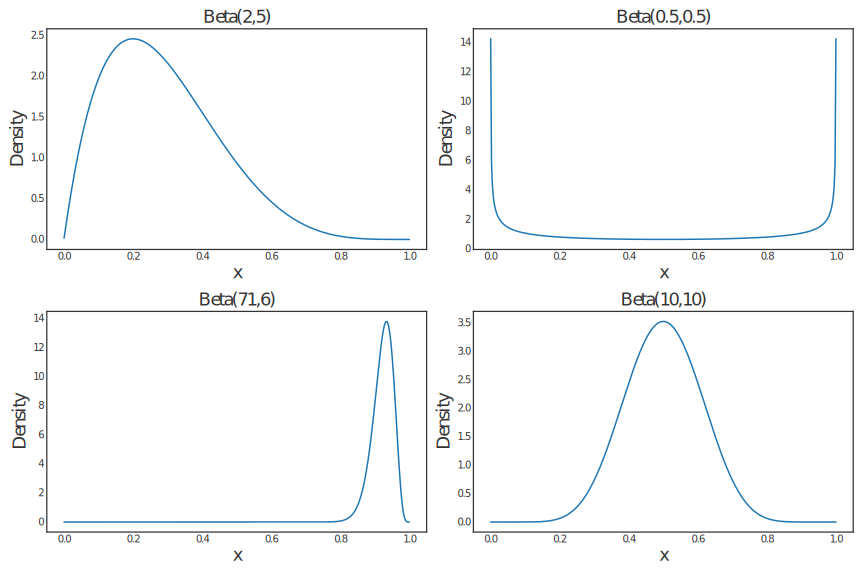
\includegraphics{images/figures/betaplot1.svg}
\caption{Plots of $\text{Beta}(a,b)$ densities for various values of $(a,b)$.}
\end{figure}

\newpage

\begin{figure}[!h]
\centering
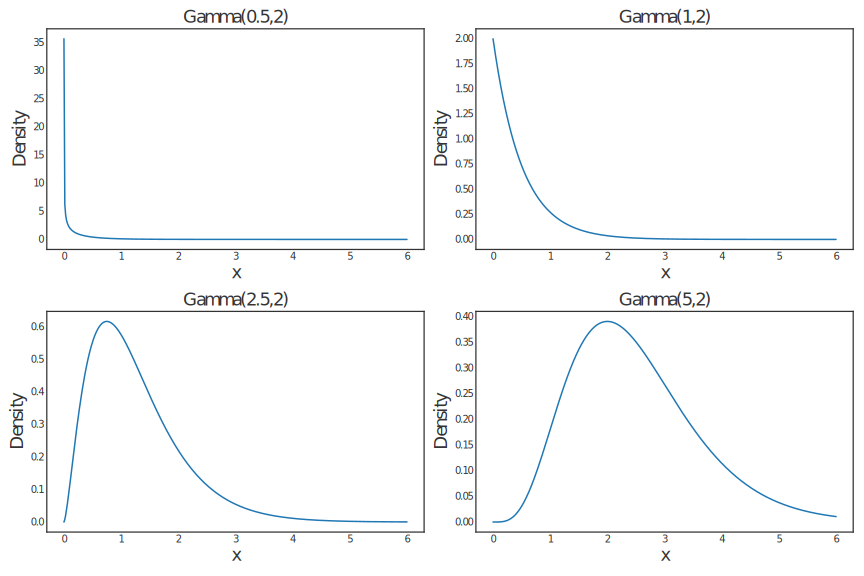
\includegraphics{images/gammaplot1.svg}
\caption{Plots of $\text{Gamma}(a,2)$ densities, for various values of $a$.}
\end{figure}

\clearpage

\section{Bayes Theorem for distributions in action}
\noindent We will now see Bayes Theorem for distributions in operation.  Remember -- for now, we will assume that someone else has provided the prior distribution for $\theta$. In Chapter 3 we will consider how this might be done.  

\paragraph{Example 2.1}{~\\
Consider an experiment with a possibly biased coin. Let
\label{ex:coin}
$\theta=\text{Pr}(\text{Head})$. Suppose that, before conducting the experiment, we believe that all values of $\theta$ are equally likely: this gives a prior distribution $\theta\sim U(0,1)$, and so
\begin{equation} 
\pi(\theta)=1,\quad\quad0<\theta<1.
\label{eq:p1}
\end{equation}
Note that with this prior distribution $\text{E}[\theta]=0.5$. We now toss the coin 5~times and observe 1~head. Determine the posterior distribution for~$\theta$ given this data.

\paragraph{Solution to Example 2.1}{

    
        The data is an observation on the random variable $X|\theta\sim
        \text{Bin}(5,\theta)$. This gives a likelihood function
        \begin{equation}
        f(x=1|\theta)=5\theta(1-\theta)^4
        \label{eq:p2}
        \end{equation}
        which favours values of $\theta$ near its maximum
        $\theta=0.2$. Therefore, we have a conflict of opinions: the prior
        distribution \eqref{eq:p1} suggests that $\theta$ is probably around
        0.5 and the data \eqref{eq:p2} suggest that it is around 0.2. We can
        use Bayes Theorem to combine these two sources of information in a
        coherent way. First
        \begin{align*}
        f(x=1) &=\int_\Theta\pi(\theta)f(x=1\, |\,\theta)\,d\theta = \int_0^1 1\times 5\theta(1-\theta)^4\,d\theta \\
        &=\int_0^1 \theta\times 5(1-\theta)^4\,d\theta =\left[-(1-\theta)^5\,\theta\right]^1_0
        +\int_0^1 (1-\theta)^5\,d\theta \\
        &=0 + \left[-\frac{(1-\theta)^6}{6}\right]^1_0 =\frac{1}{6}. 
        \end{align*}
        Therefore, the posterior density is (for $0<\theta<1$):
        \begin{align*}
        \pi(\theta|x=1)&=\frac{\pi(\theta)f(x=1|\theta)}{f(x=1)} =\frac{5\theta(1-\theta)^4}{1/6}\\
        &=30\,\theta(1-\theta)^4 =\frac{\theta(1-\theta)^4}{\mathrm{B}(2,5)},\quad\quad 0<\theta<1,
        \end{align*}
        and so the posterior distribution is $\theta|x=1\sim \textnormal{\text{Beta}}(2,5)$ -- see
        Definition~\ref{def:beta}.  This distribution has its mode at
        $\theta=0.2$, and mean at $\text{E}[\theta|x=1]=2/7=0.286$.
    
    
}


\newpage




{
    
}

\newpage

The main difficulty in calculating the posterior distribution was in obtaining the $f(x)$ term. However, in many cases we can recognise the posterior distribution without the need to calculate this constant term (constant with respect to $\theta$). In this example, we can calculate the posterior distribution as
\begin{align*}
\pi(\theta|\underline{x})&\propto\pi(\theta)f(x=1|\theta) \\
&\propto 1\times 5\theta(1-\theta)^4,\quad\quad 0<\theta<1  \\
&=k\theta(1-\theta)^4,\quad\quad 0<\theta<1.
\end{align*}
As $\theta$ is a continuous quantity, what we would like to know is what continuous distribution defined on $(0,1)$ has a probability density function which takes the form $k\theta^{g-1}(1-\theta)^{h-1}$. The answer is the $\textnormal{\text{Beta}}(g,h)$ distribution. Therefore, choosing $g$ and $h$ appropriately, we can see that the posterior distribution is $\theta|x=1\sim \textnormal{\text{Beta}}(2,5)$.

\textbf{Summary:}

It is possible that we have a biased coin. If we suppose that all values of $\theta=\text{Pr(Head)}$ are equally likely and then observe 1 head out of 5, then the most likely value of $\theta$ is 0.2 --- the same as the most likely value from the data alone (not surprising!). However, on average, we would expect $\theta$ to be around 0.286. Uncertainty about $\theta$ has changed from a (prior) standard deviation of 0.289 to a (posterior) standard deviation of 0.160. The changes in our beliefs about $\theta$ are more fully described by the prior and posterior distributions shown in Figure~\ref{fig:betaplot2}.
\begin{figure}[ht]

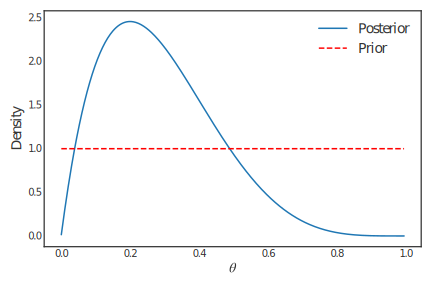
\includegraphics{images/figures/priorplot1.svg}
\caption{Prior (dashed) and posterior (solid) densities for $\theta=\text{Pr(Head)}$}
\label{fig:betaplot2}

\end{figure}}
\newpage
\paragraph{Example 2.2}{~\\
Consider an experiment to determine how good a music expert is at \label{ex:mozart} distinguishing between pages from Haydn and Mozart scores. Let $\theta=\text{Pr}(\text{correct choice})$. Suppose that, before conducting the experiment, we have been told that the expert is very competent. In fact, it is suggested that we should have a prior distribution which has a mode around $\theta=0.95$ and for which $\textnormal{Pr}(\theta<0.8)$ is very small. We choose $\theta\sim \textnormal{\text{Beta}}(77,5)$, with probability density function
\begin{equation}
\pi(\theta)=128107980\,\theta^{76}(1-\theta)^4,\quad\quad 0<\theta<1.
\label{eq:p3}
\end{equation}
A graph of this prior density is given in Figure ~\ref{fig:betaplot3}.
\begin{figure}[ht]

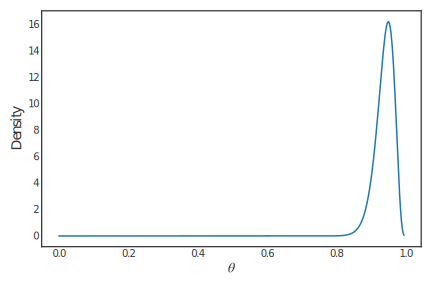
\includegraphics{images/priorplot2.svg}
\caption{Prior density for the music expert's skill.}
\label{fig:betaplot3}

\end{figure}

In the experiment, the music expert makes the correct choice 9 out of 10 times. Determine the posterior distribution for $\theta$ given this information.

\paragraph{Solution to Example 2.2}{
    
}

\newpage


{
    We have an observation on the random variable $X|\theta\sim
        \text{Bin}(10,\theta)$. This gives a likelihood function of
        \begin{equation}
        f(x=9|\theta)=10\,\theta^9(1-\theta)
        \label{eq:p4}
        \end{equation}
        which favours values of $\theta$ near its maximum $\theta=0.9$. We combine these two sources of information using Bayes Theorem. The posterior density function is 
        \begin{align}
        \label{eq:p5}
        \pi(\theta|x=9)&\propto\pi(\theta)f(x=9|\theta) \notag \\
        &\propto 128107980\,\theta^{76}(1-\theta)^4\times 10\,\theta^9(1-\theta),
        \quad\quad 0<\theta<1 \notag \\
        &=k\theta^{85}(1-\theta)^5,\quad\quad 0<\theta<1.
        \end{align}
        We can recognise this density function as one from the Beta family. So, the posterior distribution is $\theta|x=9\sim
        \textnormal{\text{Beta}}(86,6)$.
        
    
}

\textbf{Summary:}

The changes in our beliefs about $\theta$ are described by the prior and posterior distributions shown in Figure~\ref{fig:betaplot4} and summarised in Table~\ref{tab:betaplot4}.
\begin{figure}[h!]

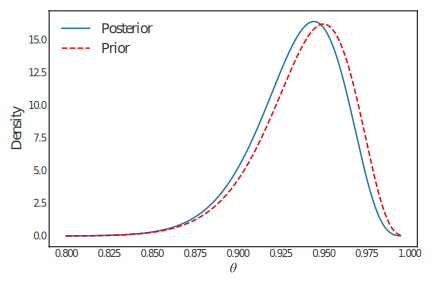
\includegraphics{images/priorposterior1.svg}
\caption{Prior (dashed) and posterior (solid) densities for the music expert's skill for the $0.8 < \theta < 1$.}
\label{fig:betaplot4}

\end{figure}
\begin{table}[h!]
\bigskip

\begin{tabular}{|l|c|c|c|}
\cline{2-4}
\multicolumn{1}{c|}{~}& Prior & Likelihood & Posterior \\
\multicolumn{1}{c|}{~}&~(\ref{eq:p3})  &~(\ref{eq:p4}) & ~(\ref{eq:p5}) \\
\hline
$\textnormal{Mode}(\theta)$ & 0.950 & 0.900 & 0.944 \\
$\text{E}[\theta]$ & 0.939 & -- & 0.935 \\
$\textnormal{SD}(\theta)$ & 0.0263 & -- & 0.0256 \\
\hline
\end{tabular}
\caption{Changes in beliefs about $\theta$.}
\label{tab:betaplot4}

\end{table}

Notice that, having observed only a 90\% success rate in the experiment, the posterior mode and mean are smaller than their prior values. Also, the experiment has largely confirmed our ideas about $\theta$, with the uncertainty about $\theta$ being only very slightly reduced.}

\newpage

\paragraph{Example 2.3}{~\\
Max, a video game pirate, is trying to identify the proportion of potential customers $\theta$ who might be interested in buying \textit{Call of Duty: Modern Warfare II} next month. \label{ex:max} Based on the proportion of customers who have bought similarly violent games from him in the past, he assumes that $\theta \sim \textnormal{\text{Beta}}(2.5,12)$; a plot of this prior density is shown in Figure \ref{fig:maxprior}.  

\begin{figure}[h!]

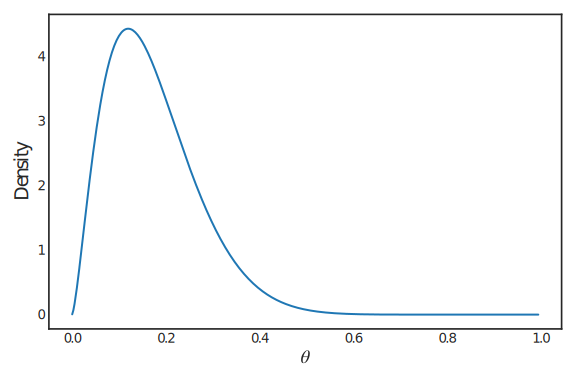
\includegraphics{images/priorplot3.svg}
\caption{Max's prior density.}
\label{fig:maxprior}

\end{figure}
Max asks five potential customers if they would buy \textit{Call of Duty: Modern Warfare II} from him, and four say they would.  Using this information, what is Max's posterior distribution for $\theta$?   
\paragraph{Solution to Example 2.3}{
    
}

{
    

    We have been told that the prior for $\theta$ is a $\text{Beta}(2.5,12)$ distribution -- this has density given by
    \begin{equation}
    \frac{1}{\mathrm{B}(2.5,12)}\theta^{2.5-1}(1-\theta)^{12-1} = 435.1867\theta^{1.5}(1-\theta)^{11}.
    \label{eq:max1}
    \end{equation}
    We have an observation on the random variable $X|\theta \sim \text{Bin}(5,\theta)$.  This gives a likelihood function of 
    \begin{equation}
    f(x=4|\theta)  = \comb{5}{4} \theta^{4}(1-\theta)^{1} = 5 \theta^{4}(1-\theta),
    \label{eq:max2}
    \end{equation}
    which favours values of $\theta$ near its maximum 0.8.  We combine our prior information (\ref{eq:max1}) with the data (\ref{eq:max2}) -- to obtain our posterior distribution -- using Bayes Theorem.  The posterior density function is
    \begin{eqnarray*}
    \pi(\theta|x=4) &\propto& \pi(\theta)f(x=4|\theta)\\
                    &\propto& 435.1867 \theta^{1.5}(1-\theta)^{11} \times 5 \theta^{4}(1-\theta), \qquad 0<\theta<1,  \\
    \end{eqnarray*}
    giving
    \begin{equation}
    \pi(\theta|x=4) = k \theta^{5.5}(1-\theta)^{12}, \qquad 0<\theta<1.
    \label{eq:max3} 
    \end{equation}
    You should recognise this density function as one from the beta family.  In fact, we have a $\text{Beta}(6.5, 13)$, i.e. $\theta|x=4 \sim \text{Beta}(6.5,13)$.  
    
    
}
\newpage

\textbf{Summary:}

The changes in our beliefs about $\theta$ are described by the prior and posterior distributions shown in Figure 2.7 and summarised in Table 2.2.
\begin{figure}[h!]

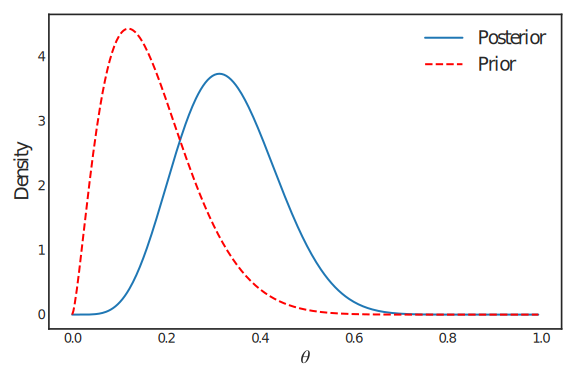
\includegraphics{images/priorposterior2.svg}
\caption{Prior (dashed) and posterior (solid) densities for Max's problem.}


\end{figure}
\begin{table}[h!]
\bigskip

\begin{tabular}{|l|c|c|c|}
\cline{2-4}
\multicolumn{1}{c|}{~}& Prior & Likelihood & Posterior \\
\multicolumn{1}{c|}{~}& (\ref{eq:max1}) & (\ref{eq:max2}) &(\ref{eq:max3}) \\
\hline
$\textnormal{Mode}(\theta)$ & 0.12 & 0.8 & 0.314 \\
$\text{E}[\theta]$ & 0.172 & -- & 0.333 \\
$\textnormal{SD}(\theta)$ & 0.096 & -- & 0.104 \\
\hline
\end{tabular}
\caption{Changes in beliefs about $\theta$.}


\end{table}

Notice how the posterior has been ``pulled'' from the prior towards the observed value: the mode has moved up from 0.12 to 0.314, and the mean has moved up from 0.172 to 0.333.  Having just one observation in the likelihood, we see that there is hardly any change in the standard deviation from prior to posterior: we would expect to see a decrease in standard deviation with the addition of more data values.}


\newpage

\paragraph{Example 2.4}{~\\
Table~\ref{tab:earth} shows some data on the times between serious \label{ex:earth} earthquakes. An earthquake is included if its magnitude is at least 7.5 on the Richter scale or if over 1000 people were killed. Recording starts on 16~December 1902 (4500 killed in Turkistan). The table includes data on 21~earthquakes, that is, 20~``waiting times'' between earthquakes. 

\begin{table}[h]
\centering
\begin{tabular}{|rrrrrrrrrr|} \hline
840&157&145&44&33&121&150&280&434&736\\
584&887&263&1901&695&294&562&721&76&710\\ \hline
\end{tabular}
\caption{Time intervals between major earthquakes (in days).}
\label{tab:earth}
\end{table}

It is believed that earthquakes happen in a random haphazard kind of way and that times between earthquakes can be described by an exponential distribution. Data over a much longer period suggest that this exponential assumption is plausible. Therefore, we will assume that these data are a random sample from an exponential distribution with rate $\theta$ (and mean $1/\theta$). The parameter $\theta$ describes the rate at which earthquakes occur. 

An expert on earthquakes has prior beliefs about the rate of earthquakes, $\theta$, described by a $\text{Gamma}(10,4000)$ distribution, which has density
density
\begin{equation}
\label{eq:earthprior}
\pi(\theta)=\frac{4000^{10}\,\theta^9e^{-4000\theta}}{\Gamma(10)}, 
\quad\theta>0, 
\end{equation}
and mean $\text{E}[\theta]=0.0025$. A plot of this prior distribution can be found in Figure~\ref{fig:earthprior}.  As you might expect, the expert believes that, realistically, only very small values of $\theta$ are likely, though larger values are not ruled out!  Determine the posterior distribution for~$\theta$.
\begin{figure}[ht]

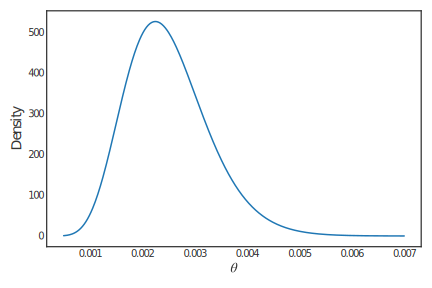
\includegraphics{images/priorplot4.svg}
\caption{Prior density for the earthquake rate $\theta$}
\label{fig:earthprior}

\end{figure}

\newpage

\paragraph{Solution to Example 2.4}{
    
    The data are observations on $X_i|\theta\sim Exp(\theta)$, $i=1,2,\ldots,20$ (independent). Therefore, the likelihood function for~$\theta$ is
    \begin{align}
    \label{eq:earthlik}
    f(\underline{x}|\theta)&=\prod_{i=1}^{20} \theta e^{-\theta x_i}, 
    \quad\quad\theta>0 \notag \\
    &=\theta^{20}\exp\left(-\theta\sum_{i=1}^{20} x_i\right),
    \quad\quad\theta>0 \notag \\
    &=\theta^{20} e^{-9633\theta},
    \quad\quad\theta>0. 
    \end{align}
    We now apply Bayes Theorem to combine the expert opinion with the observed data. The posterior density function is
    \begin{align}
    \label{eq:earthpost}
    \pi(\theta|\underline{x})&\propto\pi(\theta)f(\underline{x}|\theta) \notag \\
    &\propto\frac{4000^{10}\,\theta^{9}e^{-4000\theta}}{\Gamma(10)}\times
    \theta^{20} e^{-9633\theta},\quad\quad\theta>0 \notag  \\
    &=k\,\theta^{30-1}e^{-13633\theta},\quad\quad\theta>0.
    \end{align}
    The only continuous distribution which takes the form
    $k\theta^{g-1}e^{-h\theta}$, $\theta>0$ is the $\text{Gamma}(g,h)$ distribution.
    Therefore, the posterior distribution must be $\theta|\underline{x}\sim
    \text{Gamma}(30,13633)$.
    
    
}


\textbf{Summary:}

The data have updated our beliefs about $\theta$ from a
$\text{Gamma}(10,4000)$ distribution to a \\ $\text{Gamma}(30,13633)$ distribution. Plots of
these distributions are given in Figure~\ref{fig:earthpost}, and Table~\ref{tab:earthsum} gives a summary of the main changes induced by incorporating the data. Notice that, as the mode of the likelihood function is close to that of the prior distribution, the information in the data is consistent with that in the prior distribution. This results in a reduction in variability from the prior to the posterior distributions. The similarity between the prior beliefs and the data has reduced the uncertainty we have about the likely earthquake rate~$\theta$.

\begin{figure}[ht]

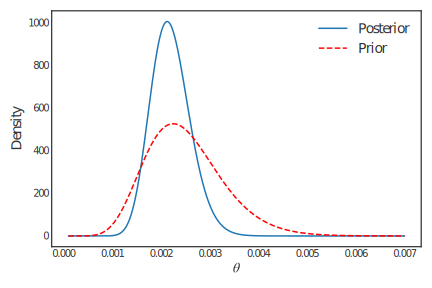
\includegraphics{images/priorposterior3.svg}
\caption{Prior (dashed) and posterior (solid) densities for the earthquake rate $\theta$.} 
\label{fig:earthpost}

\end{figure}

\begin{table}[ht]

\begin{tabular}{|l|c|c|c|}
\cline{2-4}
\multicolumn{1}{c|}{~}& Prior & Likelihood & Posterior \\
\multicolumn{1}{c|}{~}& $\eqref{eq:earthprior}$ & $\eqref{eq:earthlik}$ 
& $\eqref{eq:earthpost}$ \\
\hline
$\textnormal{Mode}(\theta)$ & 0.00225 & 0.00208 & 0.00213 \\
$\text{E}[\theta]$ & 0.00250 & -- & 0.00220 \\
$\textnormal{SD}(\theta)$ & 0.00079 & -- & 0.00040 \\
\hline
\end{tabular}
\caption{Changes in beliefs about $\theta$.}
\label{tab:earthsum}

\end{table}}

\newpage
\paragraph{Example 2.5}{~\\
  We now consider the general case of the problem discussed in Example~\ref{ex:earth}.  Suppose $X_i|\theta\sim \text{Exp}(\theta)$, $i=1,2,\ldots,n$ (independent) and our prior beliefs about $\theta$ are summarised by a $\text{Gamma}(g,h)$ distribution (with $g$ and $h$ known), with density
\begin{equation}
\label{eq:p6}
\pi(\theta)=\frac{h^g\,\theta^{g-1}e^{-h\theta}}{\Gamma(g)}, 
\quad\theta>0.
\end{equation}
Determine the posterior distribution for $\theta$.

\paragraph{Solution to Example 2.5}{
    
    The likelihood function for~$\theta$ is
    \begin{align}
    \label{eq:p7}
   f(\underline{x}|\theta)&=\prod_{i=1}^n \theta e^{-\theta x_i}, 
    \quad\quad\theta>0 \notag \\
    &= \theta^n e^{-n\bar x\theta}, \quad\quad\theta>0. 
    \end{align}
    We now apply Bayes Theorem. The posterior density function is
    \begin{align}
    \pi(\theta|\underline{x})&\propto\pi(\theta)f(\underline{x}|\theta) \notag \\
    &\propto\frac{h^g\,\theta^{g-1}e^{-h\theta}}{\Gamma(g)}\times
    \theta^n e^{-n\bar x\theta},\quad\quad\theta>0. \notag \\
    \pi(\theta|\underline{x})
    \label{eq:p8}
    &=k\theta^{g+n-1}e^{-(h+n\bar x)\theta},\quad\quad\theta>0.
    \end{align}
    where $k$ is a constant that does not depend on $\theta$. Therefore, the posterior distribution takes the form $k\theta^{g-1}e^{-h\theta}$, $\theta>0$ and so must be a gamma distribution. Thus we have $\theta|\underline{x}\sim \text{Gamma}(g+n,h+n\bar x)$.
    
    
    
}

\newpage

\textbf{Summary:} 

If we have a random sample from an $\text{Exp}(\theta)$ distribution and our prior beliefs about $\theta$ follow a $\text{Gamma}(g,h)$ distribution then, after incorporating the data, our (posterior) beliefs about $\theta$ follow a $\text{Gamma}(g+n,h+n\bar x)$ distribution.
The changes in our beliefs about $\theta$ are summarised in Table~\ref{tab:gam}, taking $g\geq 1$.
\begin{table}[!h]
\bigskip

\begin{tabular}{|l|c|c|c|}
\cline{2-4}
\multicolumn{1}{c|}{~}& Prior & Likelihood & Posterior \\
\multicolumn{1}{c|}{~}& $\eqref{eq:p6}$ & $\eqref{eq:p7}$ & $\eqref{eq:p8}$ \\
\hline
$\textnormal{Mode}(\theta)$ & $(g-1)/h$ & $1/\bar x$ & $(g+n-1)/(h+n\bar x)$ \\
$\text{E}[\theta]$ & $g/h$ & -- & $(g+n)/(h+n\bar x)$ \\
$\textnormal{SD}(\theta)$ & $\sqrt{g}/h$ & -- & $\sqrt{g+n}/(h+n\bar x)$ \\
\hline
\end{tabular}
\caption{Changes in beliefs about $\theta$.}
\label{tab:gam}

\end{table}
Notice that the posterior mean is greater than the prior mean if and only if the likelihood mode is greater than the prior mean, that is,
\begin{equation*}
\text{E}[\theta|\underline{x}]>\text{E}[\theta]\quad\iff\quad 
\textnormal{Mode}(f(\underline{x}|\theta))>\text{E}[\theta].
\end{equation*}
The standard deviation of the posterior distribution is smaller than that of the prior distribution if and only if the sample mean is large enough, that is
$$
\textnormal{SD}(\theta|\underline{x})<\textnormal{SD}(\theta)\quad\iff\quad \bar x > k.
$$}

\clearpage

\paragraph{Example 2.6}{~\\
Software engineers at \textbf{\color{darkblue}Twitter} are interested in the click-through rate $\theta$ of their advertisement recommender.

The \textbf{\color{darkblue}click-through rate} is the proportion of clicks out of the total number of impressions of an online advertisement.

The engineers assess the click-through rate by testing their recommender on users of Twitter. They obtain a total of $n$ impressions.

\begin{itemize}
\item [(a)] Using a \textbf{\color{darkblue}Beta prior}, quantify \textbf{\color{darkblue}your prior beliefs} about $\theta$.
\end{itemize}

\paragraph{Solution to Example 2.6(a)}{
    
    By plotting different Beta distributions, or by specifying $\text{E}[\theta]$ and $\text{Var}[\theta]$ and solving the system of equations to specify $a$ and $b$, I arrived at the following prior:
    $$ \theta \sim \text{Beta}(5, 100). $$
    This places the vast majority of the probability mass for values $\theta < 0.2$. I chose this because I expect that the click-through rate is very small, but I also have some uncertainty about $\theta$.
    
    
}

\begin{itemize}
\item [(b)] Specify a \textbf{\color{darkblue}probability model} for the number of successful clicks.
\end{itemize}
\paragraph{Solution to Example 2.6(b)}{
    
    In each given impression, a user either clicks on the advert or does not. A success is if the user does click on the advert. Therefore, assuming independence between each impression (which is plausible), the appropriate model is
    $$ X|\theta \sim \text{Binomial}(n, \theta), $$
    where $n$ is the total number of impressions.
    
    
}

\clearpage

\begin{itemize}
\item [(c)] Using your probability model, and a general $\theta \sim \text{Beta}(a,b)$ prior, derive the posterior distribution.
\end{itemize}
\paragraph{Solution to Example 2.6(c)}{
    
    The prior is $\theta\sim \text{Beta}(a,b)$ and so the prior pdf is
    $$ \pi(\theta) = \frac{\theta^{a-1}(1-\theta)^{b-1}}{\mathrm{B}(a,b)}.$$
    Our probability model was $X|\theta \sim \text{Binomial}(n, \theta)$. Therefore, the posterior is
    \begin{align*}
        \pi(\theta|x) &\propto \pi(\theta) f(x|\theta) \\
        &\propto \frac{\theta^{a-1}(1-\theta)^{b-1}}{\mathrm{B}(a,b)} \times \binom{n}{x} \theta^{x}(1-\theta)^{n-x} \\
        &\propto \theta^{a + x - 1} (1-\theta)^{b + n - x - 1}.
    \end{align*}
    We recognise this as the same form as the Beta pdf and we conclude that $$\theta | x \sim \text{Beta}(a + x, b + n - x).$$
    
    
}

\begin{itemize}
\item [(d)] Using your prior and the following data, derive your \textbf{\color{darkblue}posterior distribution}. Out $n=10,000$ impressions, there were 47 successful clicks.
\end{itemize}
\paragraph{Solution to Example 2.6(d)}{
    
    My prior was $\theta \sim \text{Beta}(5, 100)$. Using the update formula from part (c), with $n = 10000$ and $x = 47$, my revised belief about $\theta$ is
    $$ \theta | x \sim \text{Beta}(52, 10053). $$
    Note that $\text{E}[\theta|x] = \frac{52}{10053} = 0.00517$ (3 s.f.) and $\text{Var}[\theta|x] = 5.07\times 10^{-7}$ (3 s.f.). Due to the amount of data, the posterior is dominated by the likelihood function since the variance is so small.
    
    
}

\textbf{Summary:} 

The prior, likelihood function and posterior can be seen in Figure~\ref{fig:clickthrough}. Here, I used my prior $\theta \sim \text{Beta}(5,100)$. Our changes in belief about the click-through rate $\theta$ are summarised in Table~\ref{tab:clickthrough}, after incorporating the data.

Note how our posterior beliefs are dominated by the likelihood function. This is because we have so much data ($n = 10000$). 

\begin{figure}[h] 

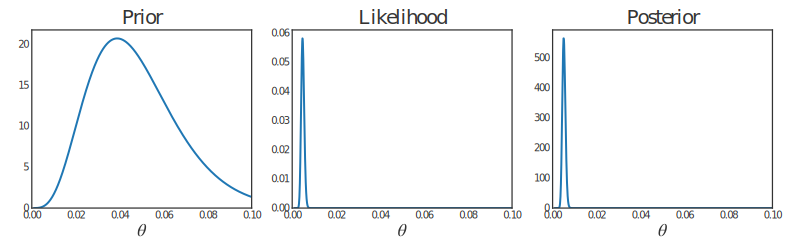
\includegraphics{images/clickthroughrate_priorposterior.svg}
\caption{Prior, likelihood function and posterior of the click-through rate $\theta$.}

\label{fig:clickthrough}
\end{figure}}

\begin{table}[!h]
\bigskip

\begin{tabular}{|l|c|c|c|}
\cline{2-4}
\multicolumn{1}{c|}{~}& Prior & Likelihood & Posterior \\
\multicolumn{1}{c|}{~}& $\eqref{eq:p6}$ & $\eqref{eq:p7}$ & $\eqref{eq:p8}$ \\
\hline
$\textnormal{Mode}(\theta)$ & $0.039$ & $ 0.0047$ & $0.005$ \\
$\text{E}[\theta]$ & $0.0476$ & -- & $0.00517$ \\
$\textnormal{SD}(\theta)$ & $0.0207$ & -- & $7.1\times 10^{-4}$ \\
\hline
\end{tabular}
\caption{Changes in beliefs about $\theta$.}
\label{tab:clickthrough}

\end{table}

\clearpage

\paragraph{Example 2.7}{~\\
You are attempting to measure the \textbf{\color{darkblue}speed of a particle} $\theta$ and quantify the uncertainty in the measurement. The experiment is set-up such that the particle \textbf{\color{darkblue}travels} $1$km and the measurements are the speed of the particle $X_i|\theta$, for $i = 1,\ldots, n$ in kilometers per second ($km/s$).

There are a \textbf{\color{darkblue}multitude of factors} that additively result in \textbf{\color{darkblue}measurement error} for the speed of the particle.

\begin{itemize}
\item [(a)] Using a \textbf{\color{darkblue}normal prior}, quantify \textbf{\color{darkblue}your prior beliefs} about $\theta$.
\end{itemize}

\paragraph{Solution to Example 2.7(a)}{
    
    Since there are physical constraints on the speed $\theta$, note that a normal prior may not be appropriate. This is because a normal distribution places probability mass over all the real line. Since we are measuring speed, we should have $0 < \theta < c$, where $c = 299792 km/s$ is the speed of light. 

    In any case, since we are asked to use a normal prior and we have no knowledge of the type of the particle being considered, a prior with little information is appropriate. For example:

    $$ \theta \sim \mathcal{N}(1.5\times 10^5, (4\times 10^4)^2).$$ 
    This places little mass outside the regions $\theta < 0$ and $\theta > c$ and does not provide much information about the speed of the particle.
    
    
    
}

\begin{itemize}
\item [(b)] Why is a \textbf{\color{darkblue}normal distribution} appropriate for the likelihood? Write down the likelihood.
\end{itemize}
\paragraph{Solution to Example 2.7(b)}{
    
    Since there an accumulation of random errors, by the central limit theorem $X_i|\theta\sim\mathcal{N}(\theta, \sigma^2)$ is a sensible model. There will also be independence between each measurement. From Example 1.7, the likelihood is
    $$ f(\underline{x}|\theta,\sigma) =  (2\pi)^{-n/2}\sigma^{-n}
        \exp\left\{-\frac{1}{2\sigma^2}
        \left(\sum_{i=1}^n x_i^2-2\theta\sum_{i=1}^n x_i+n\theta^2\right)\right\}.$$
        
    
    
}

\clearpage

\begin{itemize}
\item [(c)] Assuming that the \textbf{\color{darkblue}standard deviation} of the measurements $\sigma$ is know, derive the posterior using a general $\theta \sim \mathcal{N}(\mu_0, \sigma^2_0)$ prior.
\end{itemize}
\paragraph{Solution to Example 2.7(c)}{
    
    We will use the fact that $e^{x+y} = e^x e^y$ throughout this example. First, note that
    $$ f(\underline{x}|\theta, \sigma) \propto \exp\left\{-\frac{1}{2\sigma^2}(-2\theta n\bar{x} + n\theta^2)\right\} $$
    and
    $$ \pi(\theta) \propto \exp\left\{-\frac{1}{2\sigma^2_0}(\theta^2 - 2 \mu_0 \theta)\right\}. $$
    Therefore,
    \begin{align*}
        \pi(\theta|\underline{x}) &\propto \exp\left\{-\frac{1}{2\sigma^2}(-2\theta n\bar{x} + n\theta^2)\right\}\exp\left\{-\frac{1}{2\sigma^2_0}(\theta^2 - 2 \mu_0 \theta)\right\} \\
        &\propto \exp\left\{-\frac{1}{2}\left(\frac{n}{\sigma^2} \theta^2 - 2 \frac{n\bar{x}}{\sigma^2}\theta + \frac{\theta^2}{\sigma_0^2} - 2\frac{\mu_0}{\sigma_0^2} \theta \right)\right\} \\
        &\propto \exp\left\{-\frac{1}{2}\left(\left(\frac{n}{\sigma^2} + \frac{1}{\sigma_0^2}\right)\theta^2 - 2\left(\frac{n\bar{x}}{\sigma^2} + \frac{\mu_0}{\sigma_0^2}\right)\theta\right)\right\} \\
        &\propto \exp\left\{-\frac{1}{2}\left(\frac{\theta^2 - 2\left(\frac{n}{\sigma^2} + \frac{1}{\sigma_0^2}\right)^{-1}\left(\frac{n\bar{x}}{\sigma^2} + \frac{\mu_0}{\sigma_0^2}\right)\theta }{\left(\frac{n}{\sigma^2} + \frac{1}{\sigma_0^2}\right)^{-1}}\right)\right\}
    \end{align*}
    Let $V = \left(\frac{n}{\sigma^2} + \frac{1}{\sigma_0^2}\right)^{-1}$ and $M = \left(\frac{n}{\sigma^2} + \frac{1}{\sigma_0^2}\right)^{-1}\left(\frac{n\bar{x}}{\sigma^2} + \frac{\mu_0}{\sigma_0^2}\right)$. Then,
    \begin{align*}
        \pi(\theta|\underline{x}) &\propto \exp\left\{-\frac{1}{2V}(\theta^2 - 2M\theta)\right\} \\
        &\propto \exp\left\{-\frac{1}{2V}(\theta^2 - 2M\theta)\right\} \exp\left(-\frac{1}{2V}M^2\right) \\
        &\propto \exp\left\{-\frac{1}{2V}(\theta^2 - 2M\theta + M^2)\right\} \\
        &\propto \exp\left\{-\frac{1}{2V}(\theta - M)^2\right\}.
    \end{align*}
    We recognise this as the form of a Normal distribution with mean $M$ and variance $V$. So, 
    $$ \theta |\underline{x} \sim \mathcal{N}(M,V).$$
    
}

\clearpage

\begin{itemize}
\item [(d)] Suppose you attempted to measure the speed of the particle $4$ times and obtained the measurements (in $km/s$): 306135, 293227, 307985, 301298.

Using your prior, setting $\sigma = 5000$ and using this data, derive your \textbf{\color{darkblue}posterior distribution}.
\end{itemize}
\paragraph{Solution to Example 2.7(d)}{
    
    Using our posterior update rule from part (c) with $\bar{x} = 302161.25$, $\sigma^2 = 5000^2$, $\mu_0 = 150000$ and $\sigma_0^2 = 40000^2$, the posterior is
    $$ \theta | \underline{x} \sim \mathcal{N}(271729, 2236.068^2).$$
    
}

\textbf{Summary:}

From part (c), we know that if our data $\underline{x}$ is IID normally distributed with unknown mean $\theta$ and we choose a Normal prior distribution 
$$\theta \sim \mathcal{N}(\mu_0,\sigma^2_0)$$
to quantify our uncertainty about $\theta$, then the distribution of the posterior $\theta|\underline{x}\sim \mathcal{N}(M, V)$ is again normally distributed with mean $M$ and variance $V$, where
\begin{align*}
    M &= \left(\frac{n}{\sigma^2} + \frac{1}{\sigma_0^2}\right)^{-1}\left(\frac{n\bar{x}}{\sigma^2} + \frac{\mu_0}{\sigma_0^2}\right), \\
    V &= \left(\frac{n}{\sigma^2} + \frac{1}{\sigma_0^2}\right)^{-1}.
\end{align*}

The prior, likelihood function and posterior can be seen in Figure~\ref{fig:speed}.

\begin{figure}[h] 

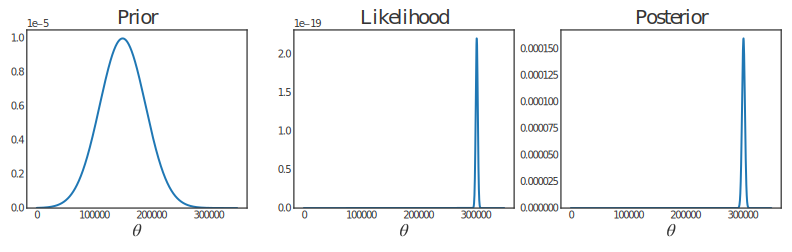
\includegraphics{images/speed_priorposterior.svg}
\caption{Prior, likelihood function and posterior of the speed of the particle $\theta$.}

\label{fig:speed}
\end{figure}}

\clearpage
\paragraph{Example 2.8}{~\\
Let $Y$ be the retreat, in feet, of the  \textit{Zachariae Isstr\o m} glacier.  A \textit{Pareto} distribution with rate $\theta$ is often used to model such geophysical activity, with probability density function 
$$
f(y|\kappa,\theta) = \theta\kappa^{\theta}y^{-(\theta+1)}, \qquad \theta,\kappa>0 \text{ and } y>\kappa.  
$$

\begin{itemize}
\item [(a)] Obtain the likelihood function for $\theta$ given the parameter $\kappa$ and some observed data $y_{1}, y_{2}, \ldots, y_{n}$ (independent).
\end{itemize}

\paragraph{Solution to Example 2.8(a)}{
    
    The likelihood function is simply the product of the probability density function evaluated at each observation $y_{i}$, ($i=1, \ldots, n$), i.e.
    \begin{align*}
    f(\underline{y} | \theta, \kappa) &= \theta\kappa^{\theta}y_{1}^{-(\theta+1)} \times \cdots \times \theta\kappa^{\theta}y_{n}^{-(\theta+1)}  \notag \\
                                   & \notag \\
                                   &= \theta^{n} \kappa^{n\theta} \prod_{i=1}^{n}y_{i}^{-(\theta+1)}.
    \end{align*}
    
    
}

\begin{itemize}
\item [(b)] Suppose we observe a retreat of 20 feet at the  \textit{Zachariae Isstr\o m} glacier in 2012.  Write down the likelihood function for $\theta$.
\end{itemize}

\paragraph{Solution to Example 2.8(b)}{
    
        We simply substitute $n=1$ and $y_{1}=20$ into the likelihood, giving
        $$
        f(\theta|\kappa,y_{1}=20)     =\theta \kappa^{\theta} 20^{-(\theta+1)}.
        $$
        
    
}

\clearpage

\begin{itemize}
\item [(c)] Using the prior $\theta \sim \text{Gamma}(9,0.36)$ for the rate of retreat and assuming $\kappa$ is known to be 12, obtain the posterior distribution $\pi(\theta|y_{1}=20)$.  
\end{itemize}

\paragraph{Solution to Example 2.8(c)}{
    
        Using Bayes Theorem, and following the examples in Chapter 2, we know that
        $$
        \pi(\theta|y_{1}=20) \propto \pi(\theta)\times f(y_1 =20 | \theta).
        $$
        Recall from Example 3.4 that our elicited prior for $\theta$ is $\text{Gamma}(9,0.36)$, which has density
        $$
        \pi(\theta) = \frac{0.36^{9}\theta^{8}e^{-0.36\theta}}{\Gamma(9)}.
        $$
        Combining this with the likelihood above (and using $\kappa=12$) gives
        \begin{align}
        \pi(\theta|y_{1}=20)   &= \frac{0.36^{9}\theta^{8}e^{-0.36\theta}}{\Gamma(9)} \times \theta 12^{\theta}20^{-(\theta+1)} \notag \\
           &  \notag \\
                               &\propto \theta^{9} e^{-0.36 \theta} 12^{\theta} 20^{-(\theta+1)}  \notag \\
            & &\notag   \\
                               &\propto \theta^{9}e^{-0.36 \theta}12^{\theta} 20^{-\theta}.
        \end{align}
        
        Now consider the term $12^{\theta}20^{-\theta}$. Taking logs, we get
        $$
        \theta \text{ln}12 - \theta \text{ln}20  = (\text{ln}12 - \text{ln}20)\theta;
        $$
        exponentiating to `re--balance', you should see that 
        $$
        12^{\theta}20^{-\theta} = e^{(\text{ln}12 - \text{ln}20)\theta}.
        $$
        Substituting back into (3.6) gives
        \begin{eqnarray*}
          \pi(\theta|y_{1}=20)  &\propto& \theta^{9}e^{-0.36 \theta} e^{(\text{ln}12 - \text{ln}20)\theta}     \qquad \text{i.e.}     \\
                   & & \\
                                &\propto& \theta^{9}e^{-0.36\theta +(\text{ln}12-\text{ln}20)\theta}    \\
                         & & \\
                                &\propto& \theta^{9}e^{-0.87 \theta}.
        \end{eqnarray*}
        Referring to our definition of the gamma distribution on page 25 of these notes, you should recognise this as a $\text{Gamma}(10,0.87)$ distribution.   
        
    
}

\newpage 

\begin{figure}[h]

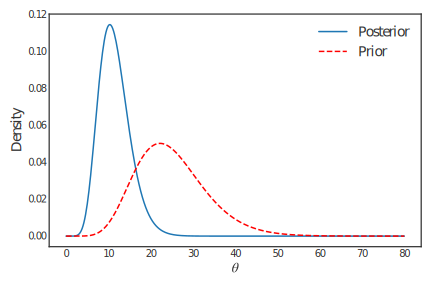
\includegraphics{images/glacier_posterior.svg}
\caption{Prior (dashed) and posterior (solid) densities for the rate of glacial retreat at the \textit{Zachariae Isstr\o m} glacier.}

\end{figure}}


\section{Conjugacy}

In Example 2.5, a gamma prior leads to a gamma posterior.
This is an example of {\it conjugacy}, where choosing a prior in a family of distributions
always leads to a posterior in the same family.
The formal definition is as follows:

\paragraph{Definition 2.4: Conjugate Prior}{~\\
Suppose that data $\underline{x}$ are modelled with distribution
$f(\underline{x}|\theta)$. A family $\mathcal{P}$ of prior distributions for
$\theta$ is \emph{conjugate} to $f(\underline{x}|\theta)$ if
for every prior distribution $\pi(\theta)\in\mathcal{P}$, the
posterior distribution $\pi(\theta|\underline{x})$ is also in $\mathcal{P}$.}

Notice that the conjugate family depends crucially on the model chosen
for the data $\underline{x}$. So we say (for example) that the Gamma distribution
is a conjugate prior for the exponential model.

There are usually simple formulae to update the conjugate prior to the corresponding posterior.
For instance, Example 2.5 showed that a $\text{Gamma}(g,h)$ prior for an exponential model
leads to a $\text{Gamma}(g+n,h+n\bar x)$ distribution.
For this reason, conjugate priors are usually a convenient choice to reduce the mathematical and computational effort of deriving the posterior.

Some examples of conjugacy are as follows:
\begin{enumerate}
\item Binomial random sample, Beta prior distribution
$\longrightarrow$ Beta posterior distribution (Examples 2.1 -- 2.3)
\item Exponential random sample, Gamma prior distribution
$\longrightarrow$ Gamma posterior distribution (Examples 2.4 -- 2.5)
\item Normal random sample (known variance), Normal prior distribution
$\longrightarrow$ Normal posterior distribution (Example 2.6)
\item $\text{Gamma}(k,\theta)$ random sample ($k$ known), Gamma prior distribution
$\longrightarrow$ Gamma posterior distribution.
\end{enumerate}

\paragraph{Example 2.9}{\label{ex:normal}~\\
Suppose we have a random sample from a normal distribution. In Bayesian statistics, when dealing with the normal distribution, the mathematics is more straightforward if we work with the precision ($=1/\text{variance}$) of the distribution rather than the variance itself. So we will assume that this population has unknown mean~$\mu$ but known precision~$\tau$. That is, 
$$X_i|\mu\sim \mathcal{N}(\mu,1/\tau),$$
for $i=1,2,\ldots,n$ (independent), where $\tau$ is known. Suppose our prior beliefs about $\mu$ can be summarised by a $\mathcal{N}(b,1/d)$ distribution, with probability density function
\begin{equation}
\label{eq:p11}
\pi(\mu)=
\left(\frac{d}{2\pi}\right)^{1/2}\exp\left\{-\frac{d}{2}(\mu-b)^2\right\}.
\end{equation}
Determine the posterior distribution for $\mu$. 

\paragraph{Solution to Example 2.9}{
    
        
    
}

\newpage

{
    
        The likelihood function for~$\mu$ is
        \begin{align*}
        f(\underline{x}|\mu)&=\prod_{i=1}^n 
        \left(\frac{\tau}{2\pi}\right)^{1/2}
        \exp\left\{-\frac{\tau}{2}(x_i-\mu)^2\right\}  \\
        &= \left(\frac{\tau}{2\pi}\right)^{n/2}
        \exp\left\{-\frac{\tau}{2}\sum_{i=1}^n (x_i-\mu)^2\right\} \\
        &= \left(\frac{\tau}{2\pi}\right)^{n/2}
        \exp\left\{-\frac{\tau}{2}\sum_{i=1}^n (x_i-\bar x+\bar x-\mu)^2\right\} \\
        &= \left(\frac{\tau}{2\pi}\right)^{n/2}
        \exp\left\{-\frac{\tau}{2}\left[\sum_{i=1}^n (x_i-\bar x)^2+n(\bar x-\mu)^2\right]\right\} 
        \end{align*}
        Let
        $$s^2 =\frac{1}{n}\sum_{i=1}^n (x_i-\bar x)^2$$
        and then
        \begin{equation}
        f(\underline{x} | \mu) = \left(\frac{\tau}{2\pi}\right)^{n/2}
        \exp\left\{-\frac{n\tau}{2}\left[s^2+(\bar x-\mu)^2\right]\right\}. \label{eq:p10}
        \end{equation}
        Applying Bayes Theorem, the posterior density function is
        \begin{align*}
        \pi(\mu|\underline{x})&\propto\pi(\mu)f(\underline{x} | \mu)\\
        &\propto \left(\frac{d}{2\pi}\right)^{1/2}\exp\left\{-\frac{d}{2}(\mu-b)^2\right\} \times \left(\frac{\tau}{2\pi}\right)^{n/2}
        \exp\left\{-\frac{n\tau}{2}\left[s^2+(\bar x-\mu)^2\right]\right\} \\
        &=k_1\exp\left\{-\frac{1}{2}\left[d(\mu-b)^2+n\tau(\bar x-\mu)^2\right]\right\}
        \end{align*}
        where $k_1$ is a constant that does not depend on $\mu$. Now the
        exponent can be simplified by expanding terms in $\mu$ and then
        completing the square, as follows.
        
    
}

\newpage

{
    
        We have
\begin{align*}
d(\mu-b)^2&+n\tau(\bar x-\mu)^2\\
&=d(\mu^2-2b\mu+b^2)+n\tau(\bar x^2-2\bar x\mu+\mu^2)\\
&=(d+n\tau)\mu^2-2(db+n\tau\bar x)\mu
+db^2+n\tau\bar x^2\\
&=(d+n\tau)\left\{\mu
-\left(\frac{db+n\tau\bar x}{d+n\tau}\right)\right\}^2+c
\end{align*}
where $c$ does not depend on $\mu$.  Let
\begin{equation}
\label{eq:p12}
B=\frac{db+n\tau\bar x}{d+n\tau}\quad\quad\text{and}\quad\quad
D=d+n\tau.
\end{equation}
Then
\begin{align}
\label{eq:p13}
\pi(\mu|\underline{x})&=k_1\exp\left\{-\frac{D}{2}(\mu-B)^2-\frac{c}{2}\right\}
\notag \\
&=k\exp\left\{-\frac{D}{2}(\mu-B)^2\right\},
\end{align}
where $k$ is a constant that does not depend on $\mu$. Therefore, the posterior distribution takes the form $k\exp\{-D(\mu-B)^2/2\}$, $-\infty<\mu<\infty$ and so must be a normal distribution: we have $\mu|\underline{x}\sim \mathcal{N}(B,1/D)$.

    
}

\newpage
\textbf{Summary:}

If we have a random sample from a $\mathcal{N}(\mu,1/\tau)$ distribution (with $\tau$ known) and our prior beliefs about $\mu$ follow a $\mathcal{N}(b,1/d)$ distribution then, after incorporating the data, our (posterior) beliefs about $\mu$ follow a $\mathcal{N}(B,1/D)$ distribution.

Notice that the way prior information and observed data combine is through the parameters of the normal distribution:
\begin{equation*}
B = \frac{db+n\tau\bar x}{d+n\tau}
\quad\quad\text{and}\quad\quad 
D = d+n\tau.
\end{equation*}
Notice also that the posterior variance (and precision) does not depend on the data, and the posterior mean is a convex combination of the prior and sample means, that is,
$$
B=\alpha b+(1-\alpha)\bar x,
$$
for some $\alpha\in(0,1)$. This equation for the posterior mean, which can be rewritten as
$$
\text{E}[\mu|\underline{x}]=\alpha \text{E}[\mu]+(1-\alpha)\bar x,
$$
arises in other models and is known as the \textit{Bayes linear rule}.

The changes in our beliefs about $\mu$ are summarised in Table~\ref{tab:norknown}.  Notice that the posterior mean is greater than the prior mean if and only if the likelihood mode (sample mean) is greater than the prior mean, that is
\begin{equation*}
\text{E}[\mu|\underline{x}] > \text{E}[\mu] \quad\iff\quad \textnormal{Mode}(f(\underline{x}|\mu))>\text{E}[\mu].
\end{equation*}
Also, the standard deviation of the posterior distribution is smaller than that of the prior distribution.

\begin{table}[ht]
\bigskip

\begin{tabular}{|l|c|c|c|}
\cline{2-4}
\multicolumn{1}{c|}{~}& Prior & Likelihood & Posterior \\
\multicolumn{1}{c|}{~}& $\eqref{eq:p11}$ & $\eqref{eq:p10}$ & $\eqref{eq:p13}$ \\
\hline
$\textnormal{Mode}(\mu)$ & $b$ & $\bar x$ & $(db+n\tau\bar x)/(d+n\tau)$ \\
$\text{E}[\mu]$ & $b$ & -- & $(db+n\tau\bar x)/(d+n\tau)$ \\
$\textnormal{Precision}(\mu)$ & $d$ & -- & $d+n\tau$ \\
\hline
\end{tabular}
\caption{Changes in beliefs about $\mu$.}
\label{tab:norknown}

\end{table}}

\newpage

\paragraph{Example 2.10}{~\\
The ages of {\it Ennerdale granophyre} rocks can be determined using \label{ex:rocks} the relative proportions of rubidium--87 and strontium--87 in the rock. An expert in the field suggests that the ages of such rocks (in millions of years) $X|\mu\sim \mathcal{N}(\mu,8^2)$ and that a prior distribution $\mu\sim \mathcal{N}(370,20^2)$ is appropriate. A rock is found whose chemical analysis yields $x=421$. What is the posterior distribution for $\mu$ and what is the probability that the rock will be older than 400 million years?

\paragraph{Solution to Example 2.10}{
    
        We have $n=1$, $\bar x=x=421$, $\tau=1/64$, $b=370$ and $d=1/400$. Therefore, we have:
        \begin{align*}
        B&=\frac{db+n\tau\bar x}{d+n\tau}
        =\frac{370/400+421/64}{1/400+1/64}=414.0\\
        D&=d+n\tau=1/400+1/64=1/7.43^2
        \end{align*}
        
        and so the posterior distribution is $\mu|x=421\sim \mathcal{N}(414.0,7.43^2)$. The (posterior) probability that the rock will be older than 400 million years is
        \begin{align*}
        Pr(\mu>400|x=421)=0.9702
        \end{align*}
        
        calculated using the $R$ commands $1-\texttt{pnorm}(400,414,7.43)$ or $1-\texttt{pnorm}(-1.884)$ or $\texttt{pnorm}(1.884)$. Without the chemical analysis, the only basis for determining the age of the rock is via the prior distribution: the (prior) probability that the rock will be older than 400 million years is $Pr(\mu>400)=0.0668$ calculated using the R command $1-\texttt{pnorm}(400,370,20)$.
        
    
}


\newpage

This highlights the benefit of taking the chemical measurements. Note that the large difference between these probabilities is not necessarily due to the expert's prior distribution being inaccurate, {\it per se}, it is probably due to the large prior uncertainty about rock ages, as shown in Figure~\ref{fig:normalplot}.
\begin{figure}[ht]

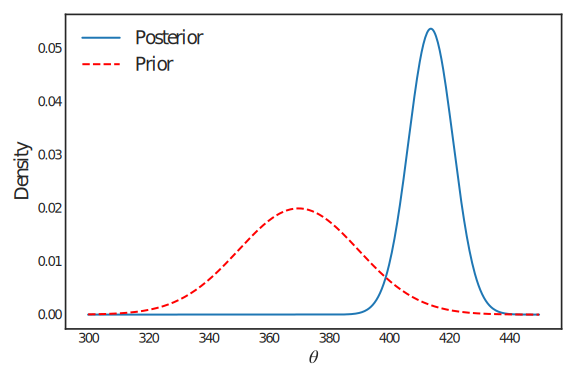
\includegraphics{images/priorposterior4.svg}
\caption{Prior (dashed) and posterior (solid) densities for the age of the rock.}
\label{fig:normalplot}

\end{figure}}

















































































































































































































































